\section{广义约化梯度法（GRG）}
\label{sec:feas-grg}

前三节都依赖集合的凸性。圆周$y^2+z^2=1$上，线段离开了约束，投影也不再有前面的性质。这时怎样从一个可行点走到另一个可行点？接下来要弄清：对光滑非线性约束，如何通过局部消元构造下降方向，又如何解方程回到约束上？

\paragraph{问题的形式}
考虑
\begin{equation}
 \min_{\bm{x}}f(\bm{x}),\qquad \bm{c}(\bm{x})=\bm{0},\quad \bm{l}\leq\bm{x}\leq\bm{u},
 \label{eq:feas-grg-problem}
\end{equation}
其中$\bm{c}:\mathbb{R}^n\to\mathbb{R}^p$连续可微，$p<n$。

不等式约束可以化成这个形式。对$g_i(\bm{x})\leq0$引入松弛变量$s_i$，改写成$g_i(\bm{x})+s_i=0$，$s_i\geq0$。例如$x_1^2+x_2^2\leq1$变成$x_1^2+x_2^2+s-1=0$，$s\geq0$。

\paragraph{主要思想}
$p$个方程把$n$个变量中的$p$个绑定了。选出$p$个变量让方程去决定，其余$n-p$个变量自由变动，约束问题就在局部变成只含自由变量的问题。这和线性规划单纯形法中“基变量由非基变量决定”的做法相同，只是这里方程非线性，决定关系是一条曲线，要靠隐函数定理保证存在，靠数值解方程求得。

\term{广义约化梯度法}（generalized reduced gradient method，GRG）依次做三件事：算自由变量上的下降方向，沿这个方向改变自由变量，再解方程把被绑定的变量拉回约束面。

\subsection{变量分块与局部消元}
\label{sec:feas-grg-partition}

选哪些变量由方程决定？选取时要满足什么条件，局部消元才成立？

\paragraph{分块}
把变量分成\term{基本变量}（basic variable）$\bm{y}\in\mathbb{R}^{p}$与\term{非基本变量}（nonbasic variable）$\bm{z}\in\mathbb{R}^{n-p}$，约束写成$\bm{c}(\bm{y},\bm{z})=\bm{0}$。对应地，把当前点的Jacobian矩阵按列分块，记
\begin{equation}
 \bm{B}=\frac{\partial\bm{c}}{\partial\bm{y}}\in\mathbb{R}^{p\times p},
 \qquad
 \bm{N}=\frac{\partial\bm{c}}{\partial\bm{z}}\in\mathbb{R}^{p\times(n-p)}.
 \label{eq:feas-grg-blocks}
\end{equation}

选择分块时有两条要求：$\bm{B}$可逆，基本变量严格位于上下界内。前者保证方程能确定$\bm{y}$，后者保证$\bm{y}$可以朝两边自由调整，用来补偿$\bm{z}$的变化。图~\ref{fig:feas-grg-partition}(a)是这种分块的示意。

\begin{BookInlineFigure}
  \centering
  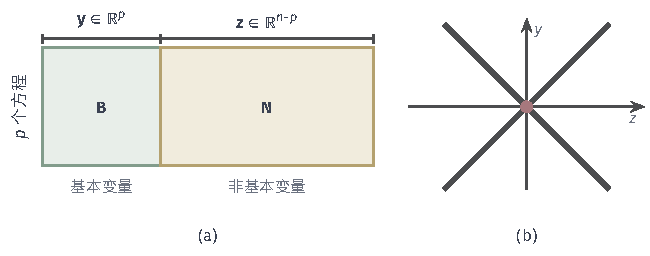
\includegraphics[width=110mm]{figures/05-optimization/06-constrained-optimization/tikz/feas-grg-partition/figure.pdf}
  \caption{局部消元的前提。(a)$p\times n$的Jacobian矩阵按变量分成可逆的方块$\bm{B}$（绿）和其余部分$\bm{N}$（黄）。(b)约束$y^2-z^2=0$的解集是两条相交直线，红点原点处的Jacobian矩阵为零，选哪个变量做基本变量都无法消元。}
  \label{fig:feas-grg-partition}
\end{BookInlineFigure}

\paragraph{局部解出基本变量}
隐函数定理说：若$\bm{c}$连续可微，$\bm{c}(\bm{y}_0,\bm{z}_0)=\bm{0}$，$\bm{B}$在该点可逆，则存在$\bm{z}_0$的邻域和其上唯一的连续可微函数$\bm{y}(\bm{z})$，满足$\bm{y}(\bm{z}_0)=\bm{y}_0$，$\bm{c}(\bm{y}(\bm{z}),\bm{z})=\bm{0}$。定理的证明可参考\BookChapterRef{chap:implicit-inverse-functions}{卷二第22章“隐函数与反函数”}。

把它代入目标，得到只含$\bm{z}$的\term{约化目标}（reduced objective）：
\begin{equation}
 F(\bm{z})=f\bigl(\bm{y}(\bm{z}),\bm{z}\bigr).
 \label{eq:feas-reduced-objective}
\end{equation}
$F$的定义只要求局部能解出$\bm{y}$，并不要求写出显式公式，也不要求全局成立。算法需要$\bm{y}(\bm{z})$的值时，就数值解一次方程。

\paragraph{例子}
本节用下面的问题贯穿：
\begin{equation}
 \min\ y,\qquad y^2+z^2=1.
 \label{eq:feas-circle}
\end{equation}
全局最优解是$(y,z)=(-1,0)$。在点$(\tfrac45,\tfrac35)$，取$y$为基本变量，$B=2y=\tfrac85$可逆，$N=2z=\tfrac65$。在这个点附近$y$由$z$决定，也就是圆周的上半弧：
\[
 y(z)=\sqrt{1-z^2},\qquad F(z)=\sqrt{1-z^2}.
\]
消元只在这一段弧上成立。到$z=\pm1$处$B=0$，上半弧到了头。

\paragraph{分块不存在的情形}
约束在某点的Jacobian矩阵行秩不足时，找不到可逆的$\bm{B}$。图~\ref{fig:feas-grg-partition}(b)的$y^2-z^2=0$在原点就是如此：解集是两条直线的交叉，附近根本不是某一个变量的函数。

基本变量都卡在界上也是一种退化：比如能使$\bm{B}$可逆的列组合都包含位于上下界的变量，这时$\bm{y}$没有双向调整的余地。这些情形需要另行处理，常用的办法有扰动、改用允许退化的换基规则，或换用第~\ref{chap:sequential-quadratic-programming}章的方法。

\subsection{约化梯度与下降方向}
\label{sec:feas-grg-gradient}

有了约化目标，它的梯度怎样算？能不能不必真正解出$\bm{y}(\bm{z})$？

\paragraph{推导}
沿约束面移动时，一阶变化$\mathrm{d}\bm{y}$和$\mathrm{d}\bm{z}$要让$\bm{c}$不变，所以
\[
 \bm{B}\,\mathrm{d}\bm{y}+\bm{N}\,\mathrm{d}\bm{z}=\bm{0}.
\]

解出基本变量的变化：
\begin{equation}
 \mathrm{d}\bm{y}=-\bm{B}^{-1}\bm{N}\,\mathrm{d}\bm{z}.
 \label{eq:feas-grg-dy}
\end{equation}

$\bm{z}$的改变不是孤立的，$\bm{y}$要跟着改变来补偿。目标的一阶变化是两部分之和：
\[
 \mathrm{d}F=\langle\nabla_{\bm{y}}f,\mathrm{d}\bm{y}\rangle+\langle\nabla_{\bm{z}}f,\mathrm{d}\bm{z}\rangle.
\]

代入式~\eqref{eq:feas-grg-dy}，把$\mathrm{d}\bm{z}$提出来，得到\term{约化梯度}（reduced gradient）：
\begin{equation}
 \nabla F=\nabla_{\bm{z}}f-\bm{N}^\top\bm{B}^{-\top}\nabla_{\bm{y}}f.
 \label{eq:feas-reduced-gradient}
\end{equation}

计算时不求逆。先解一个方阵方程$\bm{B}^\top\bm{\pi}=\nabla_{\bm{y}}f$，再算$\nabla F=\nabla_{\bm{z}}f-\bm{N}^\top\bm{\pi}$。$\bm{\pi}$是每单位约束变化的价格。线性约束、线性目标时，这个公式就是第~\ref{chap:simplex-method}章的约化成本。

\paragraph{圆周上的计算}
在式~\eqref{eq:feas-circle}中，$\nabla_yf=1$，$\nabla_zf=0$。在$(\tfrac45,\tfrac35)$，$B=\tfrac85$，$N=\tfrac65$，代入式~\eqref{eq:feas-reduced-gradient}：
\[
 \nabla F=0-\frac65\cdot\frac58\cdot1=-\frac34.
\]

用显式公式核对：$F'(z)=-z/\sqrt{1-z^2}$，在$z=\tfrac35$处正是$-\tfrac34$。

这个数的含义可以这样理解。目标本身不含$z$，$\nabla_zf=0$，单看目标似乎改变$z$没有用处。但$z$增加一点，约束的一阶变化要由$y$补偿：$\mathrm{d}y=-\tfrac34\mathrm{d}z$，而$y$就是目标。所以约化梯度记录的是“经过约束传导之后”的影响。图~\ref{fig:feas-grg-circle}画出了这个补偿三角形，以及约化目标的切线。

\begin{BookInlineFigure}
  \centering
  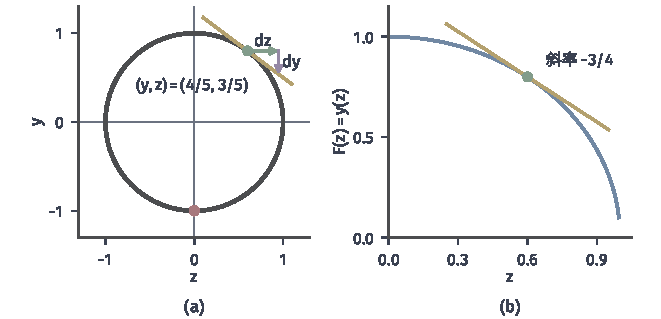
\includegraphics[width=112mm]{figures/05-optimization/06-constrained-optimization/matplotlib/feas-grg-circle/figure.pdf}
  \caption{圆周上的约化梯度。(a)深灰圆是约束，红点是最优解$(y,z)=(-1,0)$，绿点是当前点，黄线是切线；绿色箭头是$\mathrm{d}z$，紫色箭头是基本变量的一阶补偿$\mathrm{d}y=-\tfrac34\mathrm{d}z$。(b)约化目标$F(z)=\sqrt{1-z^2}$，在$z=3/5$处的切线斜率是$-3/4$。}
  \label{fig:feas-grg-circle}
\end{BookInlineFigure}

\paragraph{下降方向}
无界约束时可取$\bm{d}=-\nabla F$。非基本变量有上下界时，顶在界上又想继续往外走的坐标必须置零：
\begin{equation}
 d_j=\begin{cases}
 0,& z_j=l_j\text{ 且 }(\nabla F)_j>0,\\
 0,& z_j=u_j\text{ 且 }(\nabla F)_j<0,\\
 -(\nabla F)_j,& \text{其他}.
 \end{cases}
 \label{eq:feas-grg-direction}
\end{equation}

于是方向导数是
\[
 \langle\nabla F,\bm{d}\rangle=-\sum_{j:\,d_j\neq0}(\nabla F)_j^2.
\]
只要有一个未被置零的坐标，$\bm{d}$就是下降方向。

\subsection{可行恢复与线搜索}
\label{sec:feas-grg-restoration}

沿切向走一步之后点已经离开约束面。怎样回到约束面，又在哪里评价这一步的好坏？

\paragraph{主要思想}
固定候选的$\bm{z}^{+}=\bm{z}+\alpha\bm{d}$，把方程$\bm{c}(\bm{y},\bm{z}^{+})=\bm{0}$看成只含$\bm{y}$的$p$个方程，用Newton法求解，这个过程称为\term{可行恢复}（feasibility restoration）。切向预测$\bm{y}+\alpha\,\mathrm{d}\bm{y}$是一个已经算好的初值。

步长在恢复后的点上判断，比较$F(\bm{z}^{+})$，也就是真实可行点上的目标，而不是切线上的预测值。切线上的目标下降了，不等于回到约束面后依然下降。

\needspace{6\baselineskip}
\paragraph{变量}
\begin{itemize}
 \item $\bm{y}^{(t)}\in\mathbb{R}^p$，$\bm{z}^{(t)}\in\mathbb{R}^{n-p}$：当前基本变量与非基本变量，满足约束。
 \item $\bm{B},\bm{N}$：当前的Jacobian分块，见式~\eqref{eq:feas-grg-blocks}。
 \item $\bm{d}^{(t)}\in\mathbb{R}^{n-p}$：非基本变量的方向。
 \item $\alpha$：试探步长；$c_1\in(0,1)$：Armijo系数；$\varepsilon_c$：约束残差容差；$\varepsilon$：驻定容差。
\end{itemize}

\paragraph{初始化}
需要一个可行点和一个合格的分块。可行点本身可能要另解一个问题，例如最小化$\lVert\bm{c}(\bm{x})\rVert_2^2$。例中从式~\eqref{eq:feas-circle}的可行点出发，取$y$为基本变量，初始试探步长$\alpha=1/4$，$c_1=0.1$，$\varepsilon_c=10^{-10}$：
\[
 (y^{(0)},z^{(0)})=\bigl(\tfrac45,\tfrac35\bigr),\qquad F(z^{(0)})=0.8.
\]

\needspace{6\baselineskip}
\paragraph{每轮更新}
在第$t$轮：
\begin{enumerate}
 \item \textbf{算方向。}由式~\eqref{eq:feas-reduced-gradient}算约化梯度，由式~\eqref{eq:feas-grg-direction}得$\bm{d}^{(t)}$。若$\lVert\bm{d}^{(t)}\rVert_2\leq\varepsilon$，结束并进入第~\ref{sec:feas-grg-basis}节的检验。例中第一轮
 \[
  \nabla F=-0.75,\qquad d^{(0)}=0.75.
 \]

 \item \textbf{切向预测。}令$\bm{z}^{+}=\bm{z}^{(t)}+\alpha\bm{d}^{(t)}$，由式~\eqref{eq:feas-grg-dy}得初值
 \begin{equation}
  \bm{y}_0=\bm{y}^{(t)}-\bm{B}^{-1}\bm{N}\bigl(\bm{z}^{+}-\bm{z}^{(t)}\bigr).
  \label{eq:feas-grg-predict}
 \end{equation}
 例中第一轮
 \[
  z^{+}=0.7875,\qquad y_0=0.659375.
 \]

 \item \textbf{Newton恢复。}反复计算
 \begin{equation}
  \bm{y}_{k+1}=\bm{y}_k-\bm{B}(\bm{y}_k,\bm{z}^{+})^{-1}\bm{c}(\bm{y}_k,\bm{z}^{+}),
  \label{eq:feas-grg-newton}
 \end{equation}
 直到$\lVert\bm{c}\rVert_\infty\leq\varepsilon_c$。例中第一轮的各次结果是
 \[
  \begin{aligned}
  y_0&=0.659375, & c&=5.49\times10^{-2},\\
  y_1&=0.617721, & c&=1.74\times10^{-3},\\
  y_2&=0.616316, & c&=1.97\times10^{-6},\\
  y_3&=0.616315, & c&=2.56\times10^{-12}.
  \end{aligned}
 \]

 \item \textbf{在恢复点上做Armijo检验。}要求
 \[
  F(\bm{z}^{+})\leq F(\bm{z}^{(t)})+c_1\alpha\langle\nabla F,\bm{d}^{(t)}\rangle.
 \]
 通过就接受，否则把$\alpha$减半回到第2步。例中第一轮右端是$0.78594$，$F(z^{+})\approx0.61631$，接受。
\end{enumerate}

图~\ref{fig:feas-grg-recovery}(a)是这一轮的几何。切向预测点（空心）在圆外，Newton迭代沿竖直方向回到圆上。残差的下降呈二次收敛的样子。

\begin{BookInlineFigure}
  \centering
  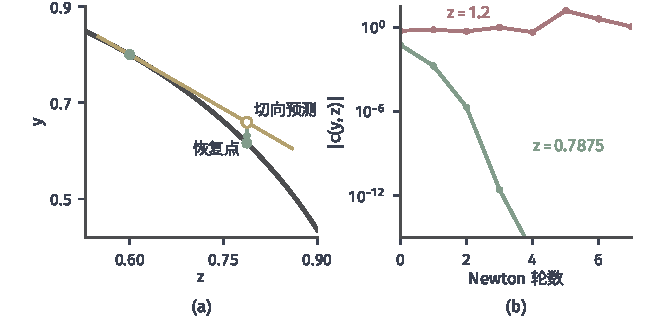
\includegraphics[width=112mm]{figures/05-optimization/06-constrained-optimization/matplotlib/feas-grg-recovery/figure.pdf}
  \caption{可行恢复。(a)从绿点沿切线（黄）走到空心点，固定$z=0.7875$后竖直回到圆周（深灰）。(b)Newton迭代中$\lvert c\rvert$的变化：绿线$z=0.7875$迅速收敛；红线$z=1.2$，方程$y^2+z^2=1$无实解，残差不减小。}
  \label{fig:feas-grg-recovery}
\end{BookInlineFigure}

例中第二轮从$(0.61632,0.7875)$出发，$\nabla F\approx-1.2778$，$d^{(1)}\approx1.2778$。先试$\alpha=\tfrac14$，得$z^{+}\approx1.1069$，超过了$1$，方程没有实解，Newton迭代的残差在几步内不降反升。

于是减半，$\alpha=\tfrac18$，$z^{+}\approx0.94722$，切向预测$y_0\approx0.41223$。Newton迭代依次给出$0.33077$、$0.32074$、$0.32059$，残差由$6.7\times10^{-2}$降到$2.5\times10^{-8}$，再一步达到容差。Armijo检验的右端约为$0.5959$，$F(z^{+})\approx0.32059$，接受：
\[
 (y^{(2)},z^{(2)})\approx(0.32059,0.94722).
\]

例中第三轮$\nabla F\approx-2.955$，方向更陡，而$z$离$1$只剩$0.053$。试探步长要连续减半四次到$\alpha=\tfrac{1}{64}$，得到$z^{+}\approx0.9934$，$y\approx0.1148$。此时$B=2y\approx0.23$已经很小，继续下去方程越来越病态，上半弧也快到头了。下一小节处理这个问题。

\paragraph{恢复失败时}
Newton迭代不收敛有几种可能的原因，处理也不同：步子太大，切向预测离约束面太远，办法是缩短$\alpha$；Jacobian矩阵过时，办法是重新计算；$\bm{B}$接近奇异，办法是换基。

恢复失败和原问题无可行解是两回事。第二轮的$z=1.1069$处方程无解，可是当前点$(0.61632,0.7875)$本身可行。恢复失败只说明这个候选的$\bm{z}^{+}$在这个分块下没有对应的可行点。

\paragraph{恢复容差与Jacobian更新}
恢复的容差要按原约束残差$\lVert\bm{c}\rVert_\infty$设置，不能按Newton步的长度设置。步长短不等于残差小，$\bm{B}$病态时尤其如此。

为了省计算，实现中常常冻结$\bm{B}$，每次Newton迭代只重新算残差。这样收敛变成线性的。第一轮冻结$B=1.6$时，残差依次是
\[
 5.49\times10^{-2},\quad1.08\times10^{-2},\quad2.42\times10^{-3},\quad5.51\times10^{-4},
\]
每次大约缩小$4.5$倍。省下分解矩阵的钱，要用更多的残差计算来付。残差下降变慢时就该更新$\bm{B}$。

\subsection{界约束与换基}
\label{sec:feas-grg-basis}

上面的例子留下两个问题：分块何时必须更换？算法停下来时，怎样判断这个点满足原问题的最优性条件？

\paragraph{一阶必要性}
第~\ref{chap:constrained-optimality}章的KKT条件要求：存在等式乘子和上下界乘子$\bm{\lambda}^{l},\bm{\lambda}^{u}\geq\bm{0}$，使Lagrange函数的梯度为零，并满足互补条件。对问题~\eqref{eq:feas-grg-problem}，这个条件可以用约化梯度来检验。

\begin{theorem}[约化梯度与KKT条件]
\label{thm:feas-grg-kkt}
设$\bm{x}=(\bm{y},\bm{z})$满足式~\eqref{eq:feas-grg-problem}的约束，$\bm{B}$可逆，$\bm{l}_{\bm{y}}<\bm{y}<\bm{u}_{\bm{y}}$。则$\bm{x}$满足KKT条件，当且仅当约化梯度~\eqref{eq:feas-reduced-gradient}的每个分量满足
\begin{equation}
 (\nabla F)_j\begin{cases}
 \geq0,& z_j=l_j,\\
 \leq0,& z_j=u_j,\\
 =0,& l_j<z_j<u_j.
 \end{cases}
 \label{eq:feas-grg-signs}
\end{equation}
此时等式乘子是$\bm{\nu}=-\bm{B}^{-\top}\nabla_{\bm{y}}f$。
\end{theorem}

\begin{proof}
KKT条件的驻定部分按两组变量写开。基本变量严格在界内，互补性使它们的上下界乘子为零，所以
\[
 \nabla_{\bm{y}}f+\bm{B}^\top\bm{\nu}=\bm{0}.
\]
$\bm{B}$可逆，这唯一地确定$\bm{\nu}=-\bm{B}^{-\top}\nabla_{\bm{y}}f$。

非基本变量的驻定条件是
\[
 \nabla_{\bm{z}}f+\bm{N}^\top\bm{\nu}-\bm{\lambda}^{l}_{\bm{z}}+\bm{\lambda}^{u}_{\bm{z}}=\bm{0}.
\]

把$\bm{\nu}$代入，前两项之和正是$\nabla F$，于是
\[
 \nabla F=\bm{\lambda}^{l}_{\bm{z}}-\bm{\lambda}^{u}_{\bm{z}}.
\]

由互补性，$z_j=l_j$时$\lambda^u_j=0$，$(\nabla F)_j=\lambda^l_j\geq0$；$z_j=u_j$时$(\nabla F)_j=-\lambda^u_j\leq0$；在界内时两个乘子都是零，$(\nabla F)_j=0$。反过来，满足式~\eqref{eq:feas-grg-signs}时，按这三种情况取乘子就得到KKT条件。
\end{proof}

用圆周例检验。加上界$z\leq\tfrac35$，点$(\tfrac45,\tfrac35)$处非基本变量在上界，$\nabla F=-\tfrac34\leq0$，符号条件成立。此时$\nu=-\tfrac58$，上界乘子是$\tfrac34$，这个点是带界问题的最优解。若没有这个上界，$\nabla F\neq0$，它就不是驻点。

\paragraph{基本变量碰界}
非基本变量的界由式~\eqref{eq:feas-grg-direction}控制，基本变量是被动的，可能在恢复时越界。例如给圆周例加上$y\geq0.7$，从$(0.8,0.6)$沿$d=0.75$前进。

用切线估计，$y$降到$0.7$的步长是$0.1/0.5625\approx0.178$。但恢复后的点在$z=0.7333$处有$y\approx0.680$，已经越界。所以步长要按恢复后的点限制，真实的碰界点在
\[
 z=\sqrt{1-0.49}\approx0.71414,\qquad\alpha\approx0.1522.
\]

这时$y$到达下界，不再满足“严格在界内”的要求，要做一次换基：$y$变成非基本变量，固定在下界；$z$变成基本变量，$B=2z\approx1.428$可逆。新的约化目标是$F(y)=y$，$\nabla F=1\geq0$，$y$在下界，条件~\eqref{eq:feas-grg-signs}成立。这个点$(0.7,0.71414)$就是带界问题的最优解。

\paragraph{基矩阵病态时换基}
即使没有碰界，$\bm{B}$接近奇异也要换基。上一小节例子的第三轮已经看到：$\lvert B\rvert$变小，约化梯度变陡，步长被压得很短。

一个简单的规则是每轮选取主元较大的变量做基本变量。圆周例只有一个方程，两列分别是$2y$和$2z$，当$\lvert y\rvert<\lvert z\rvert$时让$z$做基本变量。多个方程时，这相当于带列主元的矩阵分解选取一组条件数较好的列。图~\ref{fig:feas-grg-basis}从$(0.8,0.6)$出发，取固定步长$\alpha=1/4$。第二轮起$\lvert y\rvert<\lvert z\rvert$，基本变量换成$z$，新的约化目标$F(y)=y$的梯度是$1$，迭代沿圆周平稳越过$(y,z)=(0,1)$。等到$\lvert z\rvert<\lvert y\rvert$再换回$y$，最后收敛到$(-1,0)$。

\begin{BookInlineFigure}
  \centering
  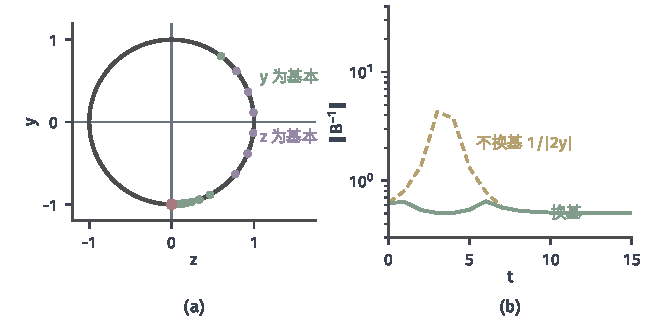
\includegraphics[width=112mm]{figures/05-optimization/06-constrained-optimization/matplotlib/feas-grg-basis/figure.pdf}
  \caption{换基的效果，问题~\eqref{eq:feas-circle}，从$(0.8,0.6)$出发，步长$1/4$。(a)迭代点的颜色表示当轮的基本变量：绿色为$y$，紫色为$z$，红点是最优解。(b)沿同一路径的$\lVert\bm{B}^{-1}\rVert$：黄色虚线是始终以$y$为基本变量时的$1/\lvert2y\rvert$，路径经过$y\approx0$附近时急剧增大；绿线是每轮换基后的值，保持有界。}
  \label{fig:feas-grg-basis}
\end{BookInlineFigure}

\paragraph{运行中要监测什么}
GRG实现要持续监测三类量：$\bm{B}$的条件数，太大就换基；原始可行性$\lVert\bm{c}(\bm{x})\rVert_\infty$和界的违反量；KKT残差，也就是式~\eqref{eq:feas-grg-signs}的违反程度。

\paragraph{每步可行不等于全局最优}
局部表示、可行恢复和换基都有条件，任何一个失败，算法就要改变动作。即使全部成功，得到的也只是满足一阶条件的点。在圆周例中，点$(y,z)=(1,0)$的约化梯度为零，它满足KKT条件，却是目标的最大点。从恰好这一点出发，方法不会移动。约束非凸时，每步可行和目标下降都推不出全局最优。
